\documentclass{libs/sig-alternate}

\usepackage{graphicx}
\usepackage{subfigure,dblfloatfix} %to fix the problem of [h!] [t!] [!b]
\usepackage{caption}

\usepackage{soul}
\usepackage[table]{xcolor} 

\usepackage[breaklinks]{hyperref}
\hypersetup{colorlinks, citecolor=blue, filecolor=black, linkcolor=blue, urlcolor=blue}

\usepackage{libs/gantt} %for the planning table
\newcommand\comment[1]{{\sffamily\textbf{[COMMENT: #1]}}}

\begin{document}

\title{<Title>}

\numberofauthors{1} 
\author{
\alignauthor
	<Your name>\\
    \affaddr{University of Twente}\\
    \email{1st author's email address}
}


\maketitle


\section*{IMPORTANT NOTES:}
Before everything, I do recommend the lecture at \url{https://www.youtube.com/watch?v=g3dkRsTqdDA}. Please, avoid vague words: relatively, possible, high, low, a lot, a few, ... Be quantitative! give an idea of numbers. Avoid start sentences with 'because'. 
	

\begin{abstract}

\comment{The structure of an average abstract should have the (i) context, (ii) problem, (iii) proposal, and your most astonishing (iv) finding. Your goal is to meet $\pm$100 words. The ``context'' part describes what your reader should know to understand your research. The ``problem'' part describes why your research need to be don; why it is interesting; and why someone needs to spend time reading your work. The ``proposal'' part describes what your approach has different from others. Finally, your ``finding'' part surprises your reader, make him VERY interested to read your paper. In a proposal you ``findings'' part describes what do you expect to be the most astonishing achievement of your research.}

\end{abstract}
\section{Proposal} \label{sec:introduction}
A Denial of Service (DoS) attack is an attack that aims to disable services of a target system. There are two main types of DoS attacks: \textit{vulnerability DoS} and \textit{flood DoS} \cite{Lin2013}. In one hand, a vulnerability DoS aims to exploit a vulnerability of a target system to reduce its performance or render it useless. An example of such an attack is to send a malformed message to the target machine which can not deal with this message and as a result stops working. On the other hand, a flood DoS attack tries to exhaust the resources of the target. An example of such an attack is to fill the entire bandwidth of the target with messages of the attacker. The attacker can accomplish such bandwidth flood by using multiple machines to produce traffic. When multiple machines are used in the attack, it is called a Distributed Denial of Service (DDoS) attack.  



%An explanation for this increase in frequency could be the rise of \textit{booters} \cite{Santana2017}. A booter, also called stressers, are websites that offer DoS attacks via a website. Booters eliminate the need for any technical knowledge to launch an attack. Clients of booters only need to pay a couple of dollars to launch an attack.

DDoS attacks have increased in power and frequency. In 2011, the peak attack was measured at 60 Gb/s \cite{Arbor2014}, in 2015, 500 Gb/s and in 2016 1.1 Tb/s \cite{Akamai2017}. In the third quartile of 2016 more than 5000 attacks where observed, whereas 200 in the entire 2012 \cite{Akamai2016}. As the number of attacks increase and downtime costs are exceeding on average \$300K per hour \cite{ITIC2016} a need for an efficient and effective mitigation method has become crucial. The first task before the mitigation is the detection of an attack. Intrusion Detection Systems (IDS) are such systems that can fulfill this task. An IDS is a system that monitors a system or network for malicious and/or suspicious activities. 
%Two main categories of IDSs are present: \textit{host-based} and \textit{network-based} \cite{Fallahi2016}. A Host-based IDS (HIDS) is only for a single machine. A Network-based IDS (NIDS) is for an entire network. A NIDS usually scans the incoming and outgoing traffic of a network endpoint. 
Based on the detection methods of IDSs, two categories can be identified: \textit{Anomaly-based} and \textit{Signature-based} \cite{fragkiadakis2015anomaly}. An Anomaly-based IDS (AIDS) bases its detection on a constructed baseline and detects deviations from this baseline. A Signature-based IDS (SIDS) bases its detection on key characteristic of an attack for which predefined signatures are known. An AIDS has as benefit that it can detect unknown attacks but with the weaknesses that it has a low accuracy, needs time to learn a baseline of a system and has difficulties to trigger alerts before an attack scales up. A SIDS has as benefit that it has a high accuracy but with the weaknesses that it is ineffective in detecting unknown attacks and it is hard to maintain an up to date signature list \cite{Liao2013}. 

Our hypothesis is that due to the high accuracy a SIDS is a suitable system that can fulfill the requirement of successfully and efficiently detecting DDoS attacks when the major downside of keeping an up to date signature list is tackled. The solution for this problem is to generate signatures for new attacks. This can be done either manually or automatically. As a manual approach requires significant amount of manual effort \cite{Lin2013}, we propose an automatic method. For this research we generate signatures from extracted features of DDoS attacks for the Bro SIDS\footnote{\url{https://www.bro.org/}}. Bro is an open source network security monitor that offers the functionality of a SIDS. The features of DDoS attacks are extracted by a different research of DDoSDB\footnote{\url{http://ddosdb.org/}}.

%We apply the to generate signatures and apply this to specific SIDS. We have chosen Bro\footnote{\url{https://www.bro.org/}} as SIDS. Bro is an open source network security monitor that offers the functionality of a SIDS. 



To pursue our goal we have defined the following research questions (RQ) as the basis of the proposed research:

%Intrusion Detection Systems (IDS) is a system that monitors a network or system for malicious and/or suspicious activities within a network or system. Two main cattogories of IDSs are present: \textit{host-based} and \textit{network-based} \cite{Fallahi2016}. A Host-based IDS (HIDS) is only for a single machine. A Network-based IDS (NIDS) is for an entire network. A NIDS usually scans the incoming and outgoing traffic of a network endpoint. Based on the detection methods of IDSs, again two categories can be identified: \textit{Anomaly-based} and \textit{Signature-based} \cite{fragkiadakis2015anomaly}. An Anomaly-based IDS (AIDS) bases its detection on a constructed baseline and detects deviations from this baseline. A Signature-based IDS (SIDS) bases its detection on signatures. An AIDS has as benefit that it can detect unknown attacks but with the weakness that it has a low accuracy and difficulty to trigger alerts in the right time. A SIDS has as benefit that it has a high accuracy but with the weakness that it is ineffective in detecting unknown attacks and it is hard to maintain an up to date signature list \cite{Liao2013}. 



%As the number of attacks are increasing and downtime costs are exceeding on average \$300K per hour \cite{ITIC2016} a need for an efficient and effective mitigation method becomes bigger. We believe that SIDSs are promising systems that can fulfil these requirements when the major downside of keeping and up to date signature list is tackled. That is why we propose an automatic method to generate signatures for the SIDS Bro\footnote{\url{https://www.bro.org/}}. To accomplish this goal we have defined the following research questions (RQ):

\begin{itemize}	
	\item \textbf{RQ1:} What are the current developments in automatic signature generation for SIDSs?
	\item \textbf{RQ2:} What is the performance of automatic signature generation against a DDoS attack for the Bro SIDS?
	 \item \textbf{RQ3:} What is the accuracy and efficiency for Bro automatic generated signatures when applied on an ongoing DDoS attack?
\end{itemize}

The first RQ will be answered by analyzing various IDSs and inspecting various signature generation methods. The second RQ will be answered by building a proof of concept that generates signatures based on a given stream of features of DDoS attacks. The third and last RQ will be answered by replaying an attack for which a signature was generated and analyze what the performance of Bro is with these signatures implemented. 





%\comment{The Introduction section has more or less the same structure as your abstract. The difference is that in the abstract each part is one statement/phrase, while in the introduction each part is a paragraph. So, (i) context, (ii) problem, (iii) proposal, and your most astonishing (iv) finding. Of course in the Introduction section you can give far more details than in the abstract. Avoid to copy and paste statements, re-write with different words.}

%\comment{In addition to the structure that you already know you should include your \textit{research questions} between the ``proposal'' paragraph and the ``findings''. The statement that precede the RQ is something like the following: }

%``To pursue our goal, we have defined the following research questions (RQ) as the basis of our research: 


%\comment{Please, avoid "yes or no" questions. Make questions that your reader are not able to answer immediately. Usually the questions depend on each other, it means that to answer one question you must answer the one before.}

%\comment{Before a little bit of your most astonishing findings you must to introduce the structure of your paper/proposal. Usually the text looks like the following.}
 
The remainder of this proposal is organized as follows. Section 2 discusses the related work identified. In Section \ref{sec:planning} we conclude with a planning for the proposed research. 



\section{Related Work}
Fallahi et. al. \cite{Fallahi2016} implemented automatic rule generation for the SIDS Snort. They used two data mining algorithms called Ripper and C5.0. They investigated five types of attacks and tested it on the ISCX 2012 dataset. Rather than looking to individual packets, they looked at the flow of data. From the flow 17 features were selected to generate rules. Fallahi et. al. applied this approach to a single dataset which contained various attacks, rather than focusing on DoS attacks. 

Fouda \cite{Fouda2017} proposes a payload based signature generation specific for DDoS attacks. Various pattern matching algorithms are tested to find the amount of similarity between incoming traffic and traffic that is associated with a DDoS attack. It was found that Smith-Waterman and Longest Common Substring algorithms yielded the highest accuracy. A problem apparent in this approach is that it tends to become slow. In 2003 IDSs could only cope with up to 200 Mbps of traffic \cite{Lai2004}. 

Chimetseren et. al \cite{Chimetseren2014} proposes signature based generation method using Discrete Fourier Transform. In this method the payload between client and server are regarded as discrete waveform. They create a spectrum for normal, known attack and unknown attack sessions.  This approach is tested on the Kyoto2006+ dataset\footnote{\url{http://www.takakura.com/Kyoto_data/}}. By also generating a spectrum for normal sessions, they are able to detect unknown attacks. However, this does yield a 5\% false positive in the selected dataset.  


\section{Proposal}

In this part I would like you to add a conceptual figure with your idea (if possible). On this, I must say that Figures MUST be in pdf format (I like to use Inkscape to create my figures, then I export to pdf) [ask me how, for help]. 

\begin{figure}[h!]
	\label{fig:approach}
	\centering
	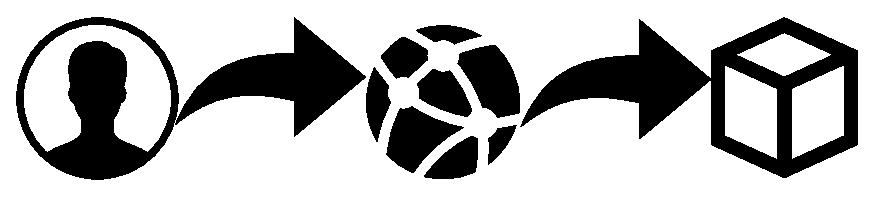
\includegraphics[width=0.5\textwidth]{figs/example.eps}
	\caption{Example of Figure.}
\end{figure}




\section{Planning tasks}\label{sec:planning}
In this section, we will briefly discuss the planning of the research. Figure \ref{fig:planning} pictures the intended planning. The first 7 weeks are planned for writing the proposal. This period knows two deadlines at the end of week 14 and 16. The first deadline is the deadline for the draft proposal and the second the deadline for the final proposal. During this period not that much time can be spent on the actual research due to other obligations. 

The remaining of the time the actual research will be carried out. During this period, more time can be spent per week in comparison to the proposal period. The research period is defined in time per RQ. The first and last RQs are more theory based and therefore probably cost less time than RQ 2 which is more practical. During RQ 3 there is also a holiday planned where no time will be spent on this research. 

Finally, a week to finalize the entire research is planned. This period is intended as a buffer in case some parts of the research are going less prosperous than intended. 


\begin{figure}[h!]
\centering
%
\noindent\resizebox{0.48\textwidth}{!}{
\begin{gantt}[xunitlength=0.5cm,fontsize=\small,titlefontsize=\small,drawledgerline=true]{10}{19} %(1)lines (2) columns
 
    \begin{ganttitle} %Month
      \titleelement{March}{4}
      \titleelement{April}{4}
      \titleelement{May}{4}
     \titleelement{June}{4}
     \titleelement{Juli}{3} 
    \end{ganttitle}
   
    \begin{ganttitle} % Week number
      \numtitle{9}{1}{27}{1}
    \end{ganttitle}

    \ganttbar{Proposal}{0}{7}
    
    \ganttgroup{RQs}{8}{10}
    \ganttbar{RQ 1}{8}{2}
    \ganttbar{RQ 2}{10}{3}
    \ganttbar{RQ 3}{13}{3}
    %\ganttbarcon[pattern=crosshatch,color=blue]{task 3}{4}{1} %(1)start point; (2) number of weeks
    %\ganttbarcon{task 4}{5}{2}  
%    \ganttcon{5}{5}{6}{6} %(1)vertical bar 

   \ganttbar[color=red]{Holidays}{14}{1}
	\ganttbar{Finalisation}{16}{1}
  
    
    \ganttmilestone{Deadlines}{6}
    \addtocounter{ganttnum}{1}
    \ganttmilestone{}{8}
    \addtocounter{ganttnum}{1}
    \ganttmilestone{}{18}
  \end{gantt}
}
\caption{Planning of this research.}
\label{fig:planning}
\end{figure}



\newpage
\bibliography{bibliography}


\end{document}
